\documentclass[dvips,11pt]{beamer}
%\documentclass[handout,dvips,11pt,grey]{beamer}
\usetheme{Goettingen}


\usepackage{tikz,pgf}
\usepackage{multicol}
\usepackage{amsmath,amsthm,amssymb}
\usepackage{epstopdf}
\usepackage{xspace}
\usepackage{verbatim}
\usepackage{sagetex}
\usepackage{circuitikz}
\usepackage{listings}
\usepackage{graphicx}
\usepackage{comment}
\usepackage{array}

\newcommand{\sizeOf}[1]{\text{{\scriptsize sizeOf}}\left( {#1} \right)}
\newcommand{\lsb}[1]{\text{{\scriptsize LSB}}\left( {#1} \right)}
\newcommand{\maxf}[2]{\text{{\scriptsize Max}}\left( {#1},{#2} \right)}
\newcommand{\maxu}[1]{\text{{\scriptsize Max}}\left( {#1} \right)}

% Ideals in the Integer Ring
% Why this is cool text
% Asymmetric Keys I
% Asymmetric Keys II


\begin{document}

\title{A Project in Modern Cryptography}

\subtitle{Homomorphic Encryption Systems}

\author{Philip M. Robinson}

%\institute{Presented to \\ Pacific Northwest National Labs}

\date{August 24, 2012}

\begin{frame}
  \titlepage
\end{frame}


\begin{frame}{Presentation Overview}

\begin{itemize}
  \item Personal Background
  \item Introduction to Homomorphic Encryption
  \item Project 
    \begin{itemize}
    \item Requirements
    \item Construction
    \item Accomplishments
    \end{itemize}
  \item Next Steps
  \item Acknowledgments
\end{itemize}

\end{frame}

\begin{frame}{Personal Background for this Project}
  \begin{itemize}
  \item BS in Computer Science from Western Washington University
  \item Cryptography and Security Hobbyist
    \begin{itemize}
      \item Kryptos
      \item CCDC
    \end{itemize}
  \item Independent Study
    \begin{itemize}
      \item Parallel Elliptic Curve Cryptography
    \end{itemize}
  \end{itemize}
\end{frame}

\begin{frame}{Why I chose this Project for this Presentation}
\begin{itemize}
\item Wide breadth of topics
\item Good team
\item New technology
\item Difficult project
\end{itemize}
\end{frame}


\begin{frame}{Definitions}
\begin{itemize}
\item Encryption - process of hiding information in a recoverable manner
\item Ciphertext - encrypted text
\item Homomorphism\hfill\(f(a\star b) = f(a)\star f(b)\)
  \begin{itemize}
    \item Partially - allows some operations
    \item Somewhat - allows all operations but has limits
    \item Fully - allows all operations
  \end{itemize}
\item Noise - distance of data from desired origin
\item Depth of circuit - how much accumulated noise a circuit produces
\end{itemize}
\end{frame} 

\begin{frame}{Introduction}
  
  \begin{itemize}
  \item What is Fully Homomorphic Encryption (FHE)

    \begin{quote}
      FHE allows arbitrary operations to be performed over encrypted data without decryption or loss of security
    \end{quote}    
      \(
      Dec(Enc(\textcolor{red}{f(}b_i\dots b_j\textcolor{red}{)}))
      \approx
      Dec(\textcolor{red}{f(}Enc(b_i)\dots Enc(b_j)\textcolor{red}{)})
      \)
      \vspace{1em}
    \item Brief history
      \begin{itemize}
        \item (Unpadded RSA) This problem was posed by Rivest 1978
          \begin{align*}
            c_1 &= m_1^e \text{mod}\;N\\
            c_2 &= m_2^e \text{mod}\;N\\
            (c_1\cdot c_2) &= \textcolor{red}{(m_1\cdot m_2)}^e\text{mod}\;N
          \end{align*}
        \item Craig Gentry 2009 (FHE)
        \item Dijk Gentry Halevi Vaikuntanathan (DGHV) cipher 2010
      \end{itemize}

  \end{itemize}
  
\end{frame}

\begin{frame}{Applications and Why this is Cool}
  \begin{itemize}
  \item Ideally you can offload sensitive computation
  \item You can trust anyone - Mail Server
  \item You can trust everyone - Distributed Nodes
    \begin{itemize}
    \item SETI@home 
    \item virtual supercomputer composed of large numbers of internet-connected nodes
    \end{itemize}
    
  \end{itemize}
  \begin{center} 
    \resizebox{3in}{!}{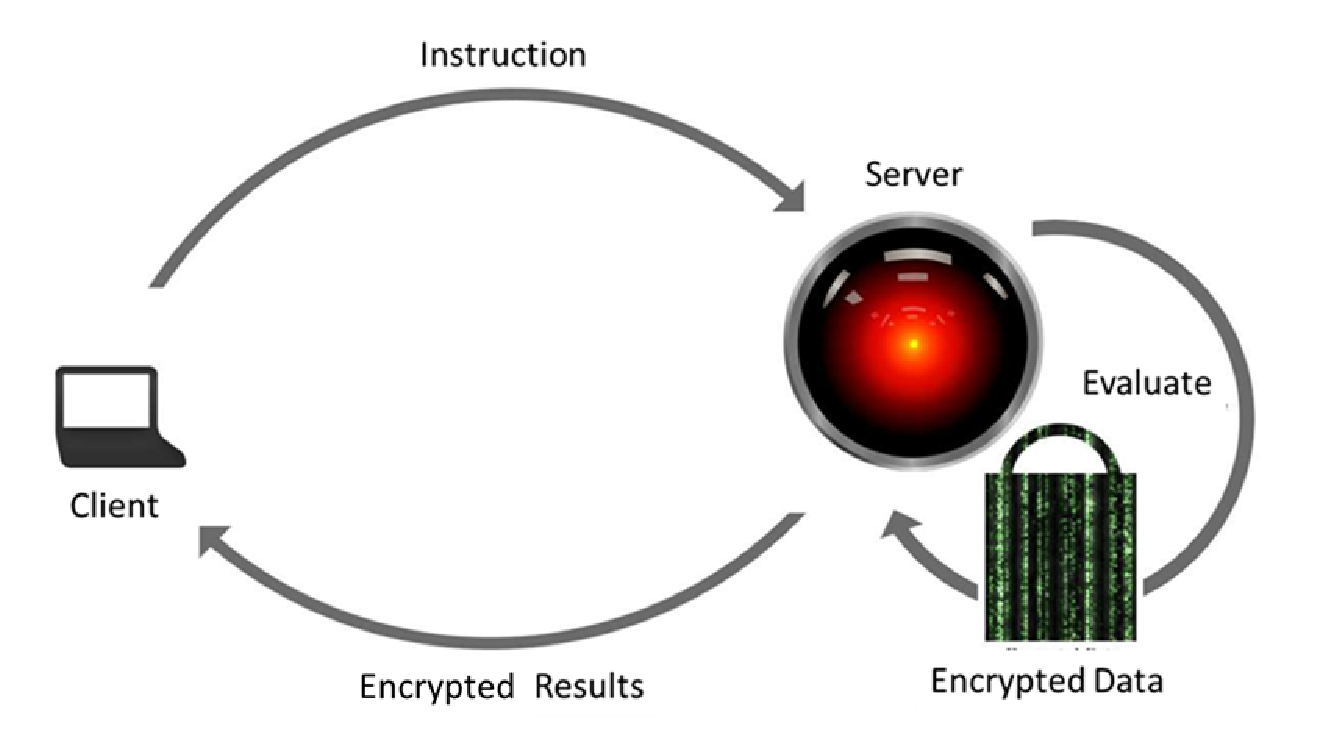
\includegraphics{image002.eps}}
  \end{center}
  
\end{frame}



\begin{frame}{Project Launch}
  \begin{itemize}
  \item Recruited Adviser
  \item Development of Course
    \begin{itemize}
    \item Syllabus
    \item Schedule
    \end{itemize}
  \item Recruited team members from competitions
  \end{itemize}
\end{frame}
  
\begin{frame}{Project Goals}
    
  \begin{itemize}
  \item Proof of Concept
  \item Product 
    \begin{itemize}    
    \item Functional
    \item Fully documented
  \end{itemize}
  \item First Uniform and Accessible Implementation 
  \end{itemize}
  
\end{frame}

\begin{frame}{Concerns Addressed}
  
  \begin{itemize}
  \item Known
    
    \begin{itemize}
    \item Steep learning curve
    \item New technology
    \item Time (9 weeks to completion)
    \end{itemize}
    
  \item Unknown
    
    \begin{itemize}
    \item Branching
    \item Data bloat - to be addressed later
    \item Time/Space complexity of 'basic' operations
    \item Network Bandwidth
    \end{itemize}
    %-------------------------
  
  \end{itemize}

\end{frame}

\begin{frame}{Project Requirements}
  \begin{itemize}
    \item Public key (Fully Homomorphic Encryption) FHE
    \item Website for computing word counts WLS
    \item Data shipping and setup will not be part of website
    \item Poster and paper
  \end{itemize}
  
  \begin{tikzpicture}
    %\draw [help lines] (0,0) grid (8,5);
    
    \node (User) at (0,0){
\includegraphics{usedcisco/mac_woman.eps}};
    \node [above] (Ulab) at (1,0){User};
    \node [scale=0.5] (Key) at (1,0) {
\includegraphics{usedcisco/key.eps}};
    
    \node [scale=0.65, left] (Text) at (1,1) {(text)};
    
    \node (WebBrowser) at (0,2) {
\includegraphics{usedcisco/web_browser.eps}};
    \node [below] (Blab) at (0,3){Browser};
    
    \node [above left,scale=0.5] (Keys) at (1,3) {
\includegraphics{usedcisco/keys.eps}};    
    \node [scale=0.65, below right] (Text) at (1,3) {Enc(text)};

    \node (WebServer) at (2,4) {
\includegraphics{usedcisco/www_server.eps}};
    \node [below] (Slab) at (2,5) {Web Server};
    \node [scale=0.65] (Slab2) at (3,4) {(Django)};
    
    \node [scale=0.9] (HadoopHead) at (4,2) {
\includegraphics{usedcisco/web_cluster}};
    \node (Hlab) at (4,1){Hadoop Cluster Head};
    
    \node (HadoopNode1) at (7,1){
\includegraphics{usedcisco/terminal.eps}};
    \node (HadoopNode2) at (7,3) {
\includegraphics{usedcisco/terminal.eps}};
    \node [scale=0.5] (HadoopNode3) at (7,2) {
\includegraphics{usedcisco/terminal.eps}};
    \node (Document) at (8,2) {
\includegraphics{usedcisco/page_icon.eps}};
    \node [below] (Nlab) at (7,4) {Hadoop Nodes};
    
    \draw [<->] (User) -- (WebBrowser);
    \draw [<->] (WebBrowser) -- (WebServer);
    \draw [<->] (WebServer) -- (HadoopHead);
    \draw [<->] (HadoopHead) -- (HadoopNode1);
    \draw [<->] (HadoopHead) -- (HadoopNode2);
    \draw [dotted] (HadoopNode1) -- (HadoopNode2);
    \draw [dotted] (HadoopNode1) -- (Document);
    \draw [dotted] (HadoopNode2) -- (Document);
    \draw [dotted] (7,2) -- (Document);
    
  \end{tikzpicture}
  

\end{frame}

\begin{frame}{Steps for Fully Homomorphic System}
  \begin{enumerate}
    \item Build a Somewhat Homomorphic System
      \begin{itemize}
        \item Bit-wise encryption rather than block-wise
        \item Well defined limits wrt. \textcolor{purple}{noise} (n)
      \end{itemize}
    \item Bootstrapping the Somewhat Homomorphic System
      \begin{itemize}
        \item {\em Size} of Decryption Circuit
        \item Circular Security
        \item \(
          Dec_0(\textcolor{red}{Enc_1(}Enc_0(b_i)
          \textcolor{red}{)},
          Enc_1(p)
          ) 
          =\textcolor{red}{Enc_1(}b_i\textcolor{red}{)}\)
      \end{itemize}
    \item Squashing the Recrypt Circuit
      \begin{itemize}
        \item Asymmetric Keys 
        \item \(
          \textcolor{red}{Rec\Big(}Enc(pk,b_i)
          +\textcolor{purple}{\text{noise}},Enc(pk,sk)\textcolor{red}{\Big)} 
          =\textcolor{red}{Enc(}pk,b_i\textcolor{red}{)}
          +\textcolor{purple}{\text{0}}\)
      \end{itemize}
    \item Distribute computing for space and time restrictions
  \end{enumerate}
\end{frame}

\begin{comment}
\begin{frame}{ Ideals of the Integer Ring }

i want to find my book 

\end{frame}
\end{comment}

\begin{frame}{How Somewhat Homomorphic System Works I}
  \begin{itemize}
  \item[\(\lambda\) :] Security Parameter is analogous to the bit-width of AES
  \item[\(b_i\) :] denotes the \(i^{th}\) `bit' of data
  \item[\(c_i\) :] denotes the cipher-text of \(b_i\)
  \item[\(n_i\) :] denotes a \(\lambda\)-bit random number corresponding to \(c_i\)

    \hspace{4em} {\em behaves as a `noise' characteristic}

  \item[\(q_i\) :] denotes a \(\lambda^5\)-bit random number corresponding to \(c_i\)

    \hspace{4em} {\em works as displacement of data}
  
  \item[\(p\) :] denotes a \(\lambda^2\)-bit random {\em odd} number (private key)
    
  \end{itemize}
  \begin{align*}
  Enc(b_i) = c_i &= p\cdot q_i + 2\cdot n_i + b_i\\
  Dec(c_i) = b_i &= \left[p\cdot q_i + 2\cdot n_i + b_i\right]_p(mod\;2)
  \end{align*}
  
\end{frame}

\begin{frame}{How Somewhat Homomorphic System Works II}
  
  \hrulefill
  
  \begin{multicols}{2}
    AND
    \resizebox{\columnwidth}{!}{
      \begin{circuitikz}\draw
        (0,0) node[and port] (myand) {}
        (myand.in 1) node[anchor=east] {{\small \({b_0}\)}}
        (myand.in 2) node[anchor=east] {{\small \({b_1}\)}}
        (myand.out) node[anchor=west] {{\small\({b_0 \cdot b_1}\;(\text{mod }2)\)}}
        ;
      \end{circuitikz}
    }\columnbreak
    \begin{align*}
      c_i\cdot c_j &= \left(p\cdot q_i + 2\cdot n_i + b_i\right)\\
      &\;\cdot\left(p\cdot q_j + 2\cdot n_j + b_j\right)\\
      &= p\cdot\hat{q} + 2\cdot\hat{n} + \left(b_i\cdot b_j\right)
    \end{align*} 
  \end{multicols}
  
  \hrulefill

  \begin{multicols}{2}
    XOR
    \resizebox{\columnwidth}{!}{
      \begin{circuitikz}\draw
        (0,0) node[xor port] (myand) {}
        (myand.in 1) node[anchor=east] {{\small\({b_0}\)}}
        (myand.in 2) node[anchor=east] {{\small\({b_1}\)}}
        (myand.out) node[anchor=west] {{\small \({b_0 + b_1}\;(\text{mod } 2)\)}}
        ;
      \end{circuitikz}
    }\columnbreak
    \begin{align*}
      c_i+ c_j &= \left(p\cdot q_i + 2\cdot n_i + b_i\right)\\
      &\;+\left(p\cdot q_j + 2\cdot n_j + b_j\right)\\  
      &= p\cdot\hat{q} + 2\cdot\hat{n} +\left(b_i+b_j\right)
    \end{align*}
    
  \end{multicols}
\hrulefill  
  
  \begin{multicols}{2}
    NOT
    \resizebox{\columnwidth}{!}{
      \begin{circuitikz}\draw
        (0,0) node[not port] (mynot) {}
        (mynot.in) node[anchor=east] {{\small\({b_0}\)}}
        (mynot.out) node[anchor=west] {{\small \({1 - b_0}\;(\text{mod } 2)\)}}
        ;
      \end{circuitikz}
    }\columnbreak
    \begin{align*}
      1 - c_i &= \left(p\cdot q_i + 2\cdot n_i + b_i\right) - 1\\
      &= p\cdot (-q_i) + 2\cdot (-n_i) +\left(1 - b_i\right)
    \end{align*}
\end{multicols}
    
\end{frame}

\begin{frame}{How Somewhat Homomorphic System Works III}
  \begin{center}
    A look at `AND' wrt. \textcolor{purple}{noise (n)}
  \end{center}
  \begin{align*}
    c_i\cdot c_j =&\left(p\cdot q_i + 2\cdot n_i + b_i\right)\cdot\left(p\cdot q_j + 2\cdot n_j + b_j\right)\\
    =&
    p\cdot(p\cdot q_i\cdot q_j + 2\cdot  q_i \cdot  n_j + 2\cdot  q_j \cdot  n_i + q_i\cdot b_j + q_j\cdot b_i)\\ 
    &+ 2\cdot \textcolor{purple}{(2\cdot n_i\cdot n_j + n_i\cdot b_j + n_j\cdot b_i)}\\
    &+ (b_i\cdot b_j)\\
    =&p\cdot\hat{q} + 2\cdot\hat{n} + \left(b_i\cdot b_j\right)
  \end{align*} 
  
  
  
  \begin{itemize}
  \item As long as \(\hat{n} < \frac{p}{2}\), then we can still correctly decrypt
  \end{itemize}
  \[
  \left.
  \begin{array}{rl}
    \stackrel{\text{{\scriptsize AND}}}{\sizeOf{\hat{n}}}&\approx2\cdot\maxf{\sizeOf{n_i}}{\sizeOf{n_j}}+3\\
    \stackrel{\text{{\scriptsize XOR}}}{\sizeOf{\hat{n}}}&\approx\maxf{\sizeOf{n_i}}{\sizeOf{n_j}}+1\\
  \end{array}
  \right\} < \big(\sizeOf{\frac{p}{2}}=\lambda^2-1\big)
  \]

\end{frame}


\begin{frame}{ Asymmetric Keys }
  
  Asymmetric keys allow us to encrypt information using {\em public keys}, and decrypt using a {\em private key}. 
  
  \begin{itemize}
  \item The public keys are a set of encrypted zeros with a few special properties
  \item The private key is the same
  \item Bootstrappable
    
    \[
    Dec_0(\textcolor{red}{Enc_1(}Enc_0(b_i)
    \textcolor{red}{)},
    Enc_1(p)
    ) 
    =\textcolor{red}{Enc_1(}b_i\textcolor{red}{)}
    \]
    
  \item Recrypt
    \[
    \textcolor{red}{Rec\Big(}Enc(pk,b_i)
    +\textcolor{purple}{\text{noise}},Enc(pk,sk)\textcolor{red}{\Big)} 
    =\textcolor{red}{Enc(}pk,b_i\textcolor{red}{)}
    +\textcolor{purple}{\text{0}}
    \]
    
    
  \end{itemize}

\end{frame}

\begin{frame}{ Recrypt } 
  
  \[Dec(c_i) = b_i = \left[p\cdot q_i + 2\cdot n_i + b_i\right]_p(mod\;2)\]

  \begin{itemize}
  \item Modulo and division circuits both use {\em division algorithm} which is too deep a circuit
  \item {\em Squashing} Circuit 
    
    \[Dec(c_i) = \lsb{c_i} \oplus \lsb{\left\lfloor\frac{c_i}{\hat{p}}\right\rceil}\]
  \item Subset Sum Problem 
    \begin{itemize}
    \item \(\hat{p}\) ends up being a vector of rationals w/ subset = \(\frac{1}{p}\)
    \item \(\hat{sk}\) is now a encrypted {0,1} vector corresponding to hamming weight of \(\hat{p}\)
    \end{itemize}
    
    %\[Dec(c_i) = c_i-\left\lfloor\sum(c_i\cdot\hat{p})\cdot\hat{sk}\right\rceil\]
    
  \end{itemize}
  
  
\end{frame}


\begin{comment}

\begin{frame}{Security of System}

Given a security parameter \(\lambda\) there exists a private key space of 

\[2^{(\lambda^2-2)} - (2^{\lambda^{2-1}})-1\]

The cryptographic hint uses the subset sum problem over a sparse subset. 

\begin{itemize}
\item[\(\lambda =\)] 8
\item[\(\beta =\)] \(8^5\)
\item[\(\alpha =\)] \(\frac{8^5}{2}\)

\end{itemize}
A brute force attack on this scheme requires an attacker to calculate \(\left(\begin{matrix}\beta\\\alpha\end{matrix}\right)\) subset sums. This would take \(2\cdot 10^{133715000000000000000}\) floating point operations; at a petaflop of computational power this would take \(2\cdot 10^{133715}\) years to brute force the private key.


\end{frame}

\end{comment}

\begin{comment}

\begin{frame}{ Asymmetric Keys }
  \begin{itemize}
    \item[\(\vec{
\includegraphics[height=1em]{usedcisco/page_icon.eps}}\)] Denotes user's input in binary form
    \item[\(\vec{
\includegraphics[height=1em]{usedcisco/keys.eps}}\)] Denotes Public Keys
    \item[\colorbox{white}{
\includegraphics[height=1em]{usedcisco/key.eps}}] Denotes Private Key or Password
    \item[\(\mathfrak{C}\)] denotes the user's desired circuit
  \end{itemize}
  \begin{center}
  \begin{tikzpicture}[auto]
    %\draw [help lines] (0,0) grid (5,5);
    
    \node[fill=green,opacity=0.5] (Alice) at (2,5) {
\includegraphics{usedcisco/standing_woman.eps}};
    
    \node[scale=0.7,fill=red,opacity=0.5] (Eve) at (2,3) {
\includegraphics{usedcisco/mac_woman.eps}};
    
    \node[scale=0.8] (Send) at (4,5) {
      \(
      \left\{
      \mathfrak{C},\text{\small Enc}
      \left(
      \vec{
\includegraphics[height=1em]{usedcisco/page_icon.eps}},
      \vec{
\includegraphics[height=1em]{usedcisco/keys.eps}}
      \right)
      \right\}
      \)
    };

    \node[scale=0.8] (Recieve) at (3,1) {
      \(
      \left\{
      \text{\small Enc}
      \left(
      \text{\small Eval}
      \left(
      \mathfrak{C},
      \vec{
\includegraphics[height=1em]{usedcisco/page_icon.eps}}
      \right),
      \vec{
\includegraphics[height=1em]{usedcisco/keys.eps}}      
      \right)
      \right\}
      \)
    };
     
    \node[scale=0.8] (Fin) at (6,3) {
\includegraphics{usedcisco/cloud.eps}};
   
    \node[fill=green,opacity=0.5] (sk) at (0,2) {
\includegraphics{usedcisco/key.eps}};
    
    \node[scale=0.8] (Dec) at (0,4) {
      \(
      \left\{
      \text{\small Eval}
      \left(
      \mathfrak{C},
      \vec{
\includegraphics[height=1em]{usedcisco/page_icon.eps}}
      \right)
      \right\}
      \)
    };    

    \draw [->,color=blue] (Alice) -- (Send) -- (Fin);
    \draw [-,color=blue] (Eve) -- (Send);
    \draw [->,color=green] (Recieve) -- (sk) -- (Dec) -- (Alice);
    \draw [->,color=red] (Fin) -- (Recieve) -- (Eve);

    
  \end{tikzpicture}
\end{center}
\end{frame}

\begin{frame}{ Asymmetric Keys II }

  \begin{itemize}  
    \item Asymmetric Key system exists
      \begin{itemize}
        \item public key is a vector of encrypted zeros with special properties
      \end{itemize}

    \item Bootstrappable
      \begin{itemize}
      \item Circular Security
      \end{itemize}
      \[
      Dec_0(\textcolor{red}{Enc_1(}Enc_0(b_i)
      \textcolor{red}{)}) 
      =\textcolor{red}{Enc_1(}b_i\textcolor{red}{)}
      \]
    \item Recrypt Exists as a small enough circuit
      \[
      \textcolor{red}{Rec\Big(}Enc(pk,b_i)
      +\textcolor{purple}{\text{noise}},Enc(pk,sk)\textcolor{red}{\Big)} 
      =\textcolor{red}{Enc(}pk,b_i\textcolor{red}{)}
      +\textcolor{purple}{\text{0}}
      \]
      \begin{itemize}
      \item Modulo and division circuits both use {\em division algorithm} which is too deep a circuit
      \item Subset Sum Problem 
        \begin{itemize}
          \item \(\hat{p}\) ends up being a vector of rationals w/ subset = \(\frac{1}{p}\)
          \item travels w/ encrypted {0,1} vector corresponding to hamming weight of \(\hat{p}\)
        \end{itemize}
      \item {\em Squashing} Circuit 

        \[Dec(c_i) = \lsb{c_i} \oplus \lsb{\left\lfloor\frac{c_i}{\hat{p}}\right\rceil}\]

      \end{itemize}
  \end{itemize}
\end{frame}


\begin{frame}{ Asymmetric Keys }
  

  \begin{itemize}
    \item[\(\vec{pk}\)] denotes public key \([pk_0 | pk_1,\dots,pk_{\lambda^6}]\)
    \item[\(sk\)] denotes secret key
      \begin{align*}
        pk_i &= sk\cdot q_i + r_i\\\\
        pk_0 &= \maxu{\vec{pk}} \\
        pk_0 &\equiv 1 \; (\text{mod}\; 2)\\
        \left[pk_0\right]_{sk} &\equiv 0 \; (\text{mod}\; 2)
      \end{align*}
  \end{itemize}

  \[Enc(b_i) = \Big( 2 \cdot ( \text{{\small randomSubsetSum}}(\vec{pk}) + n_i ) + b_i \Big) \text{ mod } pk_0 \]

\end{frame}


\begin{frame}{Decryption to Recryption Circuit}
  \[Dec(c_i,p) = b_i = \left[p\cdot q_i + 2\cdot n_i + b_i\right]_p(mod\;2)\]


  \begin{itemize}
    \item Modulo function is computed using Division algorithm 
    \item Requires secret key 
  \end{itemize}

  \[Dec(c_i) = \lsb{c_i} \oplus \lsb{\left\lfloor\frac{c_i}{p}\right\rceil}\]

  \[
  \textcolor{red}{Rec\Big(}Enc(pk,b_i)
  +\textcolor{purple}{\text{noise}},Enc(pk,sk)\textcolor{red}{\Big)} 
  \approx\textcolor{red}{Enc(}pk,b_i\textcolor{red}{)}
  +\textcolor{purple}{\text{0}}
  \]
   

\end{frame}
\end{comment}


\begin{frame}{ Voluminous Data Challenges }


  \begin{itemize}
    \item Data Bloat (decided to explore Hadoop)
      \begin{itemize}
      \item Time consequences for logic gates
      \item ``Sage-cat'' experiment (23 min)
        \begin{itemize}
        \item Fast multiplication algorithm
        \item Considered PyCuda
        \end{itemize}
      \item We spill over to Swap
      \end{itemize}
    \item PyPy 
    \item Memory Management in Python
  \end{itemize}
  \resizebox{\textwidth}{!}{
    \begin{tabular}{c|c|c|c|c|c}
      & {\small bit-size} &  {\small  volume}  & \(\lambda = 8\) & \(\lambda = 16\) & \(\lambda = 64\) \\\hline
      {\small bidgit} & 1 & \(\approx \lambda^7 \) & \(\approx\) 256 KB & 32 MB & 512 GB \\\hline
      {\small ``cadadr''} & 6 Bytes & & \(\approx\) 12 MB & 1.5 GB & 24 TB \\\hline
      {\small Dec. of Ind.} & 8.5 KB & & \(\approx\) 17 GB & 2.1 TB & 34 PB\\
    \end{tabular}
  }
  
  
\end{frame}



\begin{frame}{Hadoop}
  \begin{itemize}
  \item Hadoop 

      ``The Apache Hadoop project develops open-source software for reliable, scalable, distributed computing.''

    \begin{itemize}
    \item Map 
      \begin{itemize}
        \item Use of logic gates to implement strcmp
        %\item Binary Reduction OR
      \end{itemize}
    \item Reduce 
      \begin{itemize}
      \item Fixed width binary adder
        %\item True Zero optimization
      \end{itemize}
      
    \end{itemize} 
  \item Hadoop FS data layout
    \begin{itemize}
      \item Encrypted and split document
      \item Fixed character overlap between adjacent nodes
    \end{itemize}
  \item Circuit for word count w/ out branching 
  \end{itemize} 
\end{frame}


\begin{frame}{Optimization Implementation}
  \begin{itemize}
    \item Construction of fundamental gates to reduce noise
      \begin{center}
      \begin{circuitikz}[american ports,auto]\draw
        (0,1) node[not port,scale=0.5] (not0) {}
        (0,0) node[not port,scale=0.5] (not1) {}
        (1.5,0.5) node[and port,scale=0.5] (and0) {}
        (2,0.5) node[not port,scale=0.5] (not2) {}
        (not0.out) -| (and0.in 1)
        (not1.out) -| (and0.in 2)
        (and0.out) -| (not2.in)
        ;
      \end{circuitikz}
      %bnand(bnand(a,a),bnand(b,b))
      \begin{circuitikz}\draw
        (0,1) node[nand port,scale=0.5] (nand0) {}
        (0,0) node[nand port,scale=0.5] (nand1) {}
        (1,0.5) node[nand port,scale=0.5] (nand2) {}
        (nand0.out) -| (nand2.in 1)
        (nand1.out) -| (nand2.in 2)
        ;
      \end{circuitikz}
      \end{center}
    \item Multiplexers use binary reduction
    \item Complex circuits used in final product are fixed width
    \item True zero is used instead of encrypted zero for any possible locations
      \begin{itemize}
        \item Results in trouble w/ operations for negative numbers
        \item Allowed for {\em Jitter Multiplication}
      \end{itemize}
    \item Tail recursion and loops exclusively
    \item For testing, we had to identify which parameters could be modified
  \end{itemize}
\end{frame}


\begin{frame}{ Accomplishments }
  \begin{itemize}
  \item Highly readable code and comments
    \begin{itemize}
      \item \(2600\) lines Python
      \item Comments have citations to papers and page numbers
    \end{itemize}
  \item Public key system nearly complete
    \begin{itemize}
    \item Recrypt funny and difficult to debug
    \end{itemize}
  \item Web site sends encrypted word to Hadoop head 
  \item Hadoop cluster setup 
    \begin{itemize} 
    \item Map and reduce functions written
    \item Setup scripts written for key and data distribution
    \end{itemize}
  \item Secure systems analysis
  \item Small library of circuits for use in system
  \item Reduced 'Sage-cat' expirement to 15 min
  \end{itemize}
\end{frame}


\begin{frame}{Next Steps}
  \begin{itemize}
    \item Debug and clean up remaining features
    \item Publish article online
  \end{itemize}
  \hrulefill
  \begin{itemize}
    \item Modular reduction vs. recrypt (2010)
    \item Use of generators (Jean-Sebastien Coron)
    \item Provide code for known system attacks
    \item Currently binary model
      \begin{itemize}
      \item more compact n-ary systems
      \item ideals in vector spaces
      \end{itemize}
  \end{itemize}
  \hrulefill
  \begin{itemize}
  \item More complex user operation support
  \item Huffman codes
  \end{itemize}
\end{frame}

\begin{frame}{ Acknowledgments }

\begin{quote}I want to express my appreciation to Dr. David Bover, for overseeing this course; and my team members, for participating in this project. \end{quote}

\begin{quote}
Team members include Jeremy Caci, Ali Hajy, Jonah Jolley, Clark Rinker. \end{quote}
\end{frame}

\begin{comment}
\begin{frame}{circuit}


  \def\yr{5}
  \def\yg{4}
  \def\yx{3}
  \def\yy{1.5}
  \def\yz{0}
  \begin{circuitikz}[american ports]\draw
    node[fill=red] (ib0) at (0,\yr) {0}
    node[fill=red] (ib1) at (1,\yr) {1}
    node[fill=red] (ib2) at (2,\yr) {0}
    node[fill=red] (ib3) at (3,\yr) {0}
    node[fill=red] (ib4) at (4,\yr) {1}
    node[fill=red] (ib5) at (5,\yr) {0}
    node[fill=red] (ib6) at (6,\yr) {0}
    node[fill=red] (ib7) at (7,\yr) {1}
    ;
    \draw
    node[fill=green] (db0) at (0,\yg) {0}
    node[fill=green] (db1) at (1,\yg) {1}
    node[fill=green] (db2) at (2,\yg) {0}
    node[fill=green] (db3) at (3,\yg) {0}
    node[fill=green] (db4) at (4,\yg) {1}
    node[fill=green] (db5) at (5,\yg) {0}
    node[fill=green] (db6) at (6,\yg) {0}
    node[fill=green] (db7) at (7,\yg) {1}
    ;
    \draw
    (1.2,\yx) node[xor port, rotate=-30,scale=0.7] (xor0) {}
    (ib0) -| (xor0.in 1)
    (db0) -| (xor0.in 2)
    (2.2,\yx) node[xor port, rotate=-30,scale=0.7] (xor1) {}
    (ib1) -| (xor1.in 1)
    (db1) -| (xor1.in 2)
    (3.2,\yx) node[xor port, rotate=-30,scale=0.7] (xor2) {}
    (ib2) -| (xor2.in 1)
    (db2) -| (xor2.in 2)
    (4.2,\yx) node[xor port, rotate=-30,scale=0.7] (xor3) {}
    (ib3) -| (xor3.in 1)
    (db3) -| (xor3.in 2)
    (5.2,\yx) node[xor port, rotate=-30,scale=0.7] (xor4) {}
    (ib4) -| (xor4.in 1)
    (db4) -| (xor4.in 2)
    (6.2,\yx) node[xor port, rotate=-30,scale=0.7] (xor5) {}
    (ib5) -| (xor5.in 1)
    (db5) -| (xor5.in 2)
    (7.2,\yx) node[xor port, rotate=-30,scale=0.7] (xor6) {}
    (ib6) -| (xor6.in 1)
    (db6) -| (xor6.in 2)
    (8.2,\yx) node[xor port, rotate=-30,scale=0.7] (xor7) {}
    (ib7) -| (xor7.in 1)
    (db7) -| (xor7.in 2)
    ;
    \draw
    (2,\yy) node[or port,rotate=-90] (or0) {}
    (xor0.out) -| (or0.in 2)
    (xor1.out) -| (or0.in 1)
    (4,\yy) node[or port,rotate=-90] (or1) {}
    (xor2.out) -| (or1.in 2)
    (xor3.out) -| (or1.in 1)
    (6,\yy) node[or port,rotate=-90] (or2) {}
    (xor4.out) -| (or2.in 2)
    (xor5.out) -| (or2.in 1)
    (8,\yy) node[or port,rotate=-90] (or3) {}
    (xor6.out) -| (or3.in 2)
    (xor7.out) -| (or3.in 1)
    ;
    \draw
    (2,\yz) node[or port,scale=0.7,rotate=-135] (or4) {}
    (or0.out) -| (or4.in 2)
    (or1.out) -| (or4.in 1)
    (6,\yz) node[or port,scale=0.7,rotate=-135] (or5) {}
    (or2.out) -| (or5.in 2)
    (or3.out) -| (or5.in 1)
    ;
  \end{circuitikz}


\end{frame}
\begin{frame}{Maths 0}
      I need my abstract algebra book for this slide
  \begin{itemize}
    \item Fields
    \item Ideals
    \item Homomorphisms
  \end{itemize}
\end{frame}

\begin{frame}{Maths of Circuits I}
   Ideals of a Field
   Mapping of gates to operations in field
   Noise of operational data
\end{frame}
\begin{frame}{Maths of Circuits II}
   Noise reduction of Multiplexers and Comboplexers
   Gate transformation choices
   + show code
\end{frame}

\begin{frame}{Word Count Circuit}
  \lstinputlisting[
    language=Python,
    basicstyle=\footnotesize,
    numbers=left,
    numberstyle=\tiny\color{gray}
  ]{search.py}
\end{frame}

\end{comment}

\end{document}
